\documentclass{article}

% Pour utiliser toues les fonctions du clavier
\usepackage[utf8]{inputenc} % un package
\usepackage[T1]{fontenc}      % un second package

% Choix de la langue
\usepackage[francais]{babel}  % un troisième package
\setlength{\parindent}{0pt}

% Taille des marges
\usepackage[top=2.5cm, bottom=2cm, left=2.5cm, right=1.5cm]{geometry}

% Pour l'espace entre les lignes
\usepackage{setspace}
% Utilisation:
% Moyen:
% \begin{onehalfspace}
% \end{onehalfspace}
% Grand:
% \begin{doublespace}
% \end{doublespace}

% Changement des polices
\usepackage{charter}

% Pour afficher du code
\usepackage{verbatim}
\usepackage{moreverb}


\usepackage{titling}
\setlength{\droptitle}{-5em}   % This is your set screw

% Version 2
\usepackage{listings}

% Couleurs
\usepackage{color}
\usepackage[dvipsnames]{xcolor}
\usepackage{colortbl}

\title{%
	Laboratoires services \\
	\large Rapport laboratoire 6
}
\author{\bsc{Bulloni} Lucas \& \bsc{Wermeille} Bastien}
%\date{10 Novembre 2017}

% En-têtes et pieds de pages
\usepackage{fancyhdr}
 
\pagestyle{fancy}
\fancyhf{}
\rhead{\bsc{Bulloni} Lucas \& \bsc{Wermeille} Bastien}
\lhead{Réseau et application}
\chead{Rapport Labo 4}
\cfoot{\thepage}

% Package pour la légende de la table
\usepackage{caption}

% Package de multi-colonnes
\usepackage{multicol}

% Package pour les images
\usepackage{graphicx}

%bibliographie
\usepackage{csquotes}


% Pour les listes
\usepackage{enumitem}
\setlist[itemize]{topsep=0pt,after=\newline}

\definecolor{dkgreen}{rgb}{0,0.6,0}
\definecolor{gray}{rgb}{0.5,0.5,0.5}
\definecolor{mauve}{rgb}{0.58,0,0.82}

\lstset{frame=tb,
	language=bash,
	aboveskip=3mm,
	belowskip=3mm,
	showstringspaces=false,
	columns=flexible,
	basicstyle={\small\ttfamily},
	numbers=none,
	numberstyle=\tiny\color{gray},
	keywordstyle=\color{blue},
	commentstyle=\color{dkgreen},
	stringstyle=\color{mauve},
	breaklines=true,
	breakatwhitespace=true,
	tabsize=3
}

%affichage du titre au centre
\usepackage{titling}
\renewcommand\maketitlehooka{\null\mbox{}\vfill}
\renewcommand\maketitlehookd{\vfill\null}

%cache les liens moches
\usepackage[hidelinks]{hyperref}

\usepackage[backend=biber]{biblatex}
\addbibresource{biblio.bib}

%\bibliographystyle{plain}
\bibliography{biblio}

% Début du document
\begin{document}

\maketitle

\newpage

\tableofcontents

\newpage

\section{Introduction}
	
Dans le cadre d'un laboratoire du cours "Réseau et application", les services de base d'un réseau informatique sont mis en pratiques. Les protocoles à mettre en place sont le DHCP, DNS, serveur web et optionnellement le protocole NTP. La partie NTP a été réalisée. Le but principal est de créer un petit réseau, et ensuite 4 réseaux connectés, composé uniquement de machine GNU/Linux. Tout le laboratoire se fera sur NetKit, simulation d'environnement réseau virtuel.

\subsection{Prérequis}

\begin{itemize}
	\item Un PC Linux avec NetKit
	\item Laboratoire netkit "qos"
\end{itemize}

\subsection{Réseau du laboratoire}

\subsubsection{Réseau initial}

Le réseau est composé de deux PC, dont un qui est un serveur web, ainsi qu'un serveur qui fait office de DNS et de DHCP.\\

Le nom du réseau est net1.mylan.ch.\\

[Image sous-réseau]

\subsubsection{Réseau final}

L'objectif final est de dupliquer le premier réseau 3 fois et d'interconnecter les 4 sous-réseaux.\\

[Image réseau final]


\section{Déploiement d'un sous-réseau}

La première étape du laboratoire est la configuration du serveur DNS et DHCP. Toutes les manipulations de configurations ont été faites dans le fichier "n1-router.startup" afin que les modifications soient préservées lors du redémarrage du laboratoire.

\subsection{DHCP}

La configuration DHCP se trouvent dans la section du fichier .startup du serveur DHCP/DNS après la ligne : \\

cat >> /etc/dhcp3/dhcpd.conf << EOF

\subsubsection{Plage d'adresses dynamiques}

La première étape est la configuration de la plage d'adresse IP dynamique. Toutes les machines configurées avec une adresse IP dynamique prendront une adresse entre 192.168.1.100/24 et 192.168.1.199/24.\\

L'adresse de broadcast est 192.168.1.255 et la passerelle est 192.168.1.1. Nous avons également ajouté le serveur DNS en prévoyance. Le serveur étant la même machine que le DHCP, l'adresse est également 192.168.1.1, de ce fait, le serveur sera en adresse statique.\\

\begin{lstlisting}
subnet 192.168.1.0 netmask 255.255.255.0 {
	range 192.168.1.100 192.168.1.199;
	option routers 192.168.1.1;
	option broadcast-address 192.168.1.255;
	option domain-name-servers 192.168.1.1;
	option domain-name "net1.mylan.ch";
}
\end{lstlisting}


\subsubsection{Adresses statiques}

le serveur DNS/DHCP est configuré en IP statique, un serveur DHCP ne peut en effet pas s'attribuer une adresse dynamique. Il faut également faire attention à ne pas mettre une adresse statique dans la plage d'adresse dynamique pour ne pas créer de conflit. La configuration du serveur DHCP est faite dans la définition de la zone de la partie précédente\\

Le serveur web est également configuré avec une adresse IP statique. En effet, un serveur Web ne va que très rarement changer d'adresse IP afin d'éviter des problèmes de mise à jour DNS. Nous avons décidé de donner l'adresse 192.168.1.42 pour ce serveur. La configuration est la suivante : \\

\begin{lstlisting}
host tournedix {
	hardware ethernet	00:00:00:01:00:00;
	fixed-address		192.168.1.42;
}
\end{lstlisting}

\subsection{DNS}

La configuration DNS est également faite dans le fichier .startup du serveur.

\subsubsection{Définition de la zone}

Comme énoncé précédemment, la zone (sous-réseau) est composé d'un serveur web et d'un PC simple, et d'un serveur DHCP/DNS. Comme le protocole l'énonce, les entrées DNS sont de type NS, les entrées simples A (pour IPv4), les alias CNAME et les serveurs mails MX. \cite{cours}\\

Certaines entrées doivent être configurées dans les deux sens, du passage de l'hostname à l'adresse IP et de l'adresse IP à l'hostname.\\

la configuration hostname vers adresse ip est faite après la ligne : \\
'cat > /var/lib/bind/net1.mylan.ch.zone << EOF' \\

Et la configuration hostname vers adresse IP est faite après la ligne :\\
 'cat > /var/lib/bind/1.168.192.in-addr.arpa.zone << EOF'

\paragraph{Serveur DNS/DHCP}

Comme énoncé précédemment, le serveur DNS doit être de type NS. Mais cet enregistrement ne permet pas de spécifier son hostname, il faut donc également ajouter une adresse de type A pour pouvoir y accéder via son hostname. Un alias a également été fait pour que la machine puisse être accédé avec le nom 'routeur' et 'dns'.\\

La configuration est donc la suivante : 

\begin{lstlisting}
@	IN	NS	dns.net1.mylan.ch.
dns	IN	A	192.168.1.1
@	IN	A	192.168.1.1
routeur	IN	CNAME	dns
\end{lstlisting}

et dans l'autre zone :

\begin{lstlisting}
@	IN 	NS	dns.net1.mylan.ch.
\end{lstlisting}

\paragraph{Serveur Web}

Le serveur web sera accessible avec le nom www et pc1. Deux enregistrement de type A ont donc été fait : \\

\begin{lstlisting}
pc1	IN	A	192.168.1.42
www	IN	A	192.168.1.42
\end{lstlisting}

Il faut également faire la correspondance inverse afin d'y accéder avec l'adresse complète (URL). La configuration est comme ceci : 

\begin{lstlisting}
42	IN	PTR	www.net1.mylan.ch.
\end{lstlisting}

\paragraph{Serveur mail}

Il a également fallu configuré une entrée DNS de type MX pour chaque PC mais avec une priorité différente.

\begin{itemize}
	\item pc1 : Priorité 0
	\item pc2 : Priorité 10
\end{itemize}

La configuration est la suivante : 

\begin{lstlisting}
@	IN	MX	0	pc1
@	IN	MX	10	pc2.net1.mylan.ch.
\end{lstlisting}

\subsubsection{Tests}

\paragraph{DHCP Dynamique}

Sur la prise d'écran ci-dessous, on peut remarqué que pc2 a bien pris une adresse dans la plage 192.168.1.100/24 - 192.168.1.199/24. La machine ayant pris l'adresse 192.168.1.101. L'adresse 192.168.1.100 n'a pas été pris car au moment du teste, pc1 était aussi en adresse dynamique.

\begin{figure}[!ht]
	\centering
	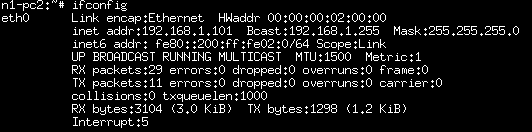
\includegraphics{./captures/testpc2-dhcp.png}
	\caption{Test DHCP dynamique}
	\label{fig:Test DHCP dynamiqu}
\end{figure}

\paragraph{DHCP Statique}

On a également testé l'adresse fixe pour pc1. Le tout étant fonctionnel :

\begin{figure}[!ht]
	\centering
	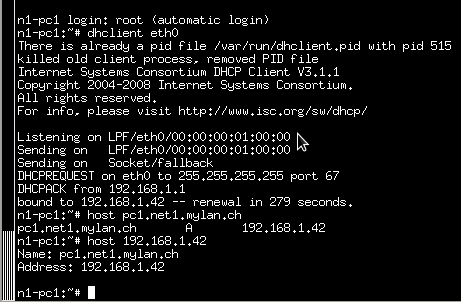
\includegraphics{./captures/7-testfixadress.png}
	\caption{Test DHCP statique pour pc1}
	\label{fig:Test DHCP statique pour pc1}
\end{figure}

Le log du serveur DHCP a également été vérifié afin d'être sûr qu'il n'y ait pas d'erreur.

\begin{figure}[!ht]
	\centering
	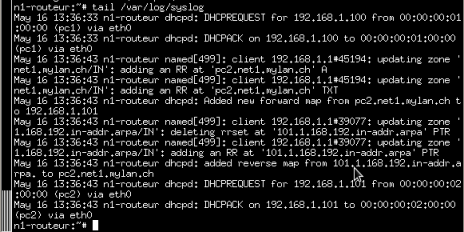
\includegraphics{./captures/2-log-dhcp.png}
	\caption{Log DHCP}
	\label{fig:Log DHCP}
\end{figure}

\paragraph{DNS}

Sur l'image ci-dessous on peut voir que les entrées DNS de la zone et que le serveur DNS est bien configuré correctement.

\begin{figure}[!ht]
	\centering
	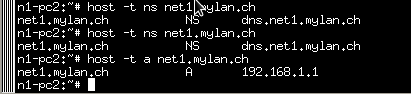
\includegraphics{./captures/1-testrouteur-dns1-pc2.png}
	\caption{Test DNS serveur}
	\label{fig:Test DNS serveur}
\end{figure}

Et sur l'image suivante que le l'alias pour le routeur est également fonctionnel.

\begin{figure}[!ht]
	\centering
	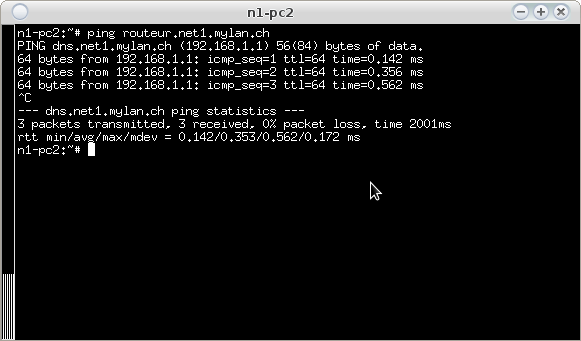
\includegraphics{./captures/alias-routeur.png}
	\caption{Test alias}
	\label{fig:Test alias}
\end{figure}

Les testes des entrées pour pc1 et pc2 ont également été fait et sont un succès comme on peut le constaté sur l'image ci-dessous.

\begin{figure}[!ht]
	\centering
	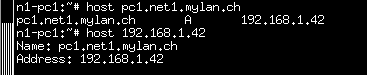
\includegraphics{./captures/2-test-dns-pc1.png}
	\caption{Test entrées DNS pc}
	\label{fig:Test entrées DNS pc}
\end{figure}

L'image montre uniquement un test sur pc1 mais un teste à également été fait sur pc2 et produit le même résultat avec les bonnes adresses IP et hostname.

\paragraph{Serveur web}

Le serveur web a été testé avec le commande 'Lynx' comme énoncé dans le document du laboratoire et le test est aussi un succès. \cite{doc-labo}

\begin{figure}[!ht]
	\centering
	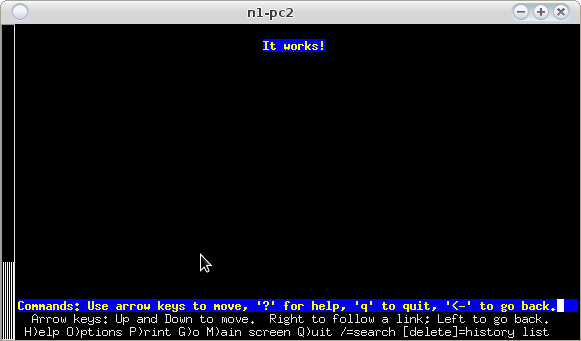
\includegraphics{./captures/ItWorks-www.png}
	\caption{Serveur Web}
	\label{fig:Serveur Web}
\end{figure}

\subsubsection{Champs TXT}

Le champ TXT est un simplement des informations textuelles sur le serveur. Ce champ TXT générer automatique contient. \cite{TXT}\\

L'entrée générée ci-dessous contient un hash qui permet de vérifier l'authenticité du DNS.

\begin{figure}[!ht]
	\centering
	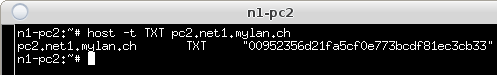
\includegraphics{./captures/txt-entry.png}
	\caption{Entrée TXT}
	\label{fig:Entrée TXT}
\end{figure}

\section{Déploiement de 4 sous-réseaux}

L'étape suivante est de dupliquer le sous-réseau 3 fois et les interconnectés. Les routeurs auront donc deux interfaces. Une pour le réseau internet et une autre pour l'accès aux autres réseaux. Ces interfaces seront d'adresse 192.168.0.X/24.\\

Le routage entre les différents sous-réseaux est fait avec Zebra, logiciel qui s'occupe de faire du routage TCP/IP \cite{Zebra}. Mais le logiciel semble ne plus être maintenu et a été remplacé par Quagga. Mais Zebra a quand même été utilisé car c'était le logiciel inclus dans le laboratoire.

\section{Autres services}

PTP text du cours:
Le protocole PTP (Precision Time Protocol ), coupe a du support dans les équipements de commutation permettant de modifier les datagrammes couche 4 en transit (transparent clock) et d'y insérer des informations de délais effectifs, peut atteindre la précision requise, dans la mesure ou les délais peuvent être estimées symétriques et constants durant les fenêtres de synchronisation. Un des avantages du
PTP est la possibilité, si les équipements de commutation le supportent (boundary clock), de pouvoir supporter la synchronisation en phase.

\section{Questions}

\subsection*{1. Quel est le rôle du mot clé authoritative dans la configuration du serveur DHCP ?}
Dans le cas où l'on a configuré le sous-réseau ```aa.bb``` dans le DHCP, une requête venant d'un sous-réseau "non identifié" ```aa.bb.cc``` sera ignorée si ce mot clé n'est pas activé, s'il est activé, le serveur répondra avec un NACK

\subsection*{2. Pour quelle raison aurait-on tendance à configurer une durée de bail DHCP courte (p.ex. 1h) ? ou longue ? (p.ex. 1 semaine)}
\begin{itemize}
\item bail court: quand il y a beaucoup de clients et pas beaucoup d'adresses IP disponibles dans la plage
\item bail long: quand il y a de grandes plages d'adresses IP et pas beaucoup de clients
\end{itemize}

\subsection*{3. Peut-on imaginer un réseau dans lequel aucune adresse de type hard static n’existe ?}
Non, il faut au moins que le routeur ait une adresse hard static, afin que les différents périphériques puissent joindre le serveur.
TODO check

\subsection*{4. Quel est l’avantage de configurer des imprimantes, machines virtuelles ou éventuellement serveurs en adresse de type DHCP static ?}
Ces périphériques sont toujours censés être disponibles! Les mettre en adresse dynamique n'apporte rien. Ces périphériques doivent être en adresse statique afin de toujours pouvoir être atteint de la même manière. Certains programmes par exemple sauvegardent l'adresse IP de certains serveurs au lieu du nom, ce qui poserait des problèmes peur ceux-ci. La configuration statique permet également de limiter le nombre de requêtes inutiles à chaque changement d'adresse des ces différents serveurs/imprimantes/...

\subsection*{5. Peut-on mettre les plages d’adresses DHCP dynamiques là où se trouvent des adresses hard static ?}
Non, le serveur DHCP risquerait d'allouer dynamiquement une adresse statique déjà allouée. Si nous voulions pouvoir faire cette manipulation qui n'apporte pas grand-chose, il faudrait que le serveur DHCP sache que ces adresses sont déjà allouées ce qui revient à modifier la plage d'adresses DHCP disponible pour allocation.

\subsection*{6. Qu’est-ce que Cisco appelle des manual bindings ?}
Ce sont des adresses IP (un pool) liées à certaines adresses MAC connues par le serveur DHCP.

TODO completer

\subsection*{7. Expliquez le concept derrière la configuration DNS suivante (faites abstraction du CNAME, mais tenez compte du TTL et du fait qu’il y a 2 champs A différents) :}
```
\$ dig -t a www.yahoo.com
www.yahoo.com.            216   IN    CNAME   fd-fp3.wg1.b.yahoo.c
fd-fp3.wg1.b.yahoo.com.   38    IN    A       46.228.47.114
fd-fp3.wg1.b.yahoo.com.   38    IN    A       46.228.47.115

\#lancez plusieurs fois la commande pour voir si quelque chose change
```
on a un serveur dupliqué donc deux serveurs à disposition. Cela permet de répartir la charge sur plusieurs serveurs différents et d'avoir de la redondance en cas de panne.

\subsection*{8. Consultez sur un serveur DHCP le fichier ```/var/lib/DHCP/dhcpd.leases``` : que contient-il ? qu’en déduisez-vous sur la volatilité des adresses IP dynamiques ?}
Contiens les bails DHCP. Les adresses IP dynamiques qui ont été allouées possèdent une "durée de vie" limitée qui expire au bout d'un certain moment. Une fois le bail expiré, celui-ci est supprimé et le périphérique qui possédait e bail doit en redemander un.

\subsection*{9. Capturez et expliquez ce qui se passe avec : ```host big-entry.alphanet.ch``` (sur machine réelle, ou ```nslookup```)}
Il y de nombreuses adresses IP qui s'affichent:
```
big-entry.alphanet.ch has address 192.168.24.25
```

il y a plusieurs serveurs physiques qui répondent à ce nom (plusieurs entrées avec le même nom dans la résolution d'adresses directe DNS)

TODO ...

\subsection*{10. Expliquez la résolution inverse (adresse IP vers nom)}
Correspond à la résolution inverse, d’ adresse IP vers nom.

\subsection*{11. Comment un serveur de nom trouve-t-il quels serveurs gèrent la racine ```.``` ?}
Le nombre de serveurs racines est limité dans le monde et ceux-ci sont codés en dur.

TODO Check

\subsection*{12. A quoi sert l’option DNS (bind/named) ```forwarders``` ?}
L'option “forwarders” permet de rediriger les requêtes qui ne sont pas résolues par notre serveur vers un serveur DNS distant (serveurs DNS de votre FAI par exemple).

Cela permet d'utiliser le cache d'un serveur déjà existant et donc d'obtenir des temps d'accès plus rapides. Si la requête DNS n'est pas résolue par le serveur DNS “distant” alors la requête sera envoyée aux serveurs DNS racine.

\subsection*{13. Vous modifiez une zone gérée par un master et un slave DNS, que devez-vous absolument changer ?}
Il est nécessaire de mettre à jour les informations des 2 serveurs DNS, du master et du slave.

\subsection*{14. Que pensez-vous de la sécurité du protocole DNS ? Quelles possibilités existent pour l’améliorer ?}
Ce protocole n'est pas sûr et possède plusieurs problèmes de sécurité tel le "DNS Spoofing", qui permet de rediriger les requêtes vers des "faux sites". Il existe une version sécurisée de ce protocole, DNSSEC qui est comme DNS, mais qui inclut du cryptage.

\subsection*{15. Vous venez de configurer deux serveurs DNS pour la zone ```mondomaine.ch```, et ils sont associés à un registrar : expliquez ce que le registry 1 doit faire pour que cela fonctionne, techniquement (indication : ```whois alphanet.ch``` ; de plus, voir les entrées ```NS``` sur ```n1-routeur``` de ```mylan.ch``` vers les sous-domaines)}
Faire remonter l'existence de ce réseau au DNS supérieur qui s'occupe de la zone.

\subsection*{16. Pourquoi est-ce important d’avoir des champs PTR existants et cohérents ?}
\begin{itemize}
\item Faciliter le changement de configuration
\item Sécurité
\end{itemize}
TODO développer

\subsection*{17. A quoi servent les champs de type SRV ? et TXT ? et NAPTR ? (donnez un exemple pour chacun)}
\begin{itemize}
\item SRV : indique quel serveur s'occupe d'un service spécifique : SIP
\item TXT : texte libre. Exemple: notification de règles SPF (Shortest Path First)
\item NAPTR : conversion de valeurs. Exemple: n\degre de téléphone en URI SIP
\end{itemize}

\subsection*{18. A-t-il été nécessaire de changer le protocole DNS pour supporter les domaines accentués, ou seule une modification du client a suffi ? (indication : punycode, exemple : ```linux-neuchâtel.ch``` dans votre navigateur)}
\begin{itemize}
\item Aucune modification du DNS
\i,tem Mais utilisation de punycode
\end{itemize}

\subsection*{19. A quoi sert le DNSSEC ?}
Sécuriser le protocole `DNS` avec l'ajout d'un chiffrement des données.



\section{Questions pour le rapport}
\subsection*{1. Expliquez ce que l’on doit faire sur le maître et le secondaire pour activer un secondaire (slave)}
Il est nécessaire de référencer le serveur DNS slave dans le fichier de configuration du routeur principal et référencer le serveur maître dans le secondaire.

\subsection*{2. Sécurité d’un serveur de nom}
Indications,  \url{http://docstore.mik.ua/orelly/networking_2ndEd/dns/ch11_02.htm}

\subsubsection*{(a) Pourquoi les serveurs récursifs sont-ils dangereux ?}
Car un attaquant peut faire une attaque de type "DNS Spoofing" sans avoir à se trouver dans le réseau. Il peut faire une requête DNS au roteur vers site dont il veut détourner le trafic et immédiatement après envoyer des réponses DNS au serveur DNS avec une réponse pour ce site avec l'adresse IP de son site malveillant.

Cela lui permet de faire croire à l'utilisateur qu'il se trouve sur le site qu'il a demandé alors qu'il ne l'est pas.

\subsubsection*{(b) Pourquoi est-ce une bonne pratique de séparer les serveurs autoritaires d’une zone sur Internet d’un serveur récursif pour un sous-réseau ?}
Afin que le serveur récursif ne soit accessible que depuis le sous-réseau et pas depuis l'extérieur. Cela permet de limiter les attaques par spoofing.

\subsubsection*{(c) Qu’est-ce qu’une attaque de trafic amplification sur le DNS ? Comment l’éviter ?}
Il s'agit d'envoyer des paquets DNS à des serveurs récursifs ouverts avec comme provenance l'adresse du serveur à attaquer. La requête DNS pourrait être \textit{dig ANY isc.org @x.x.x.x}. Cette requête de 64 bytes peut retourner environ 3'223 bytes, ce qui correspond à une multiplication du  trafic(amplification) par 50.\\

Le comble de ce problème et que la requête en question est possible grave au protocole DNSSEC qui permet d'améliorer la sécurité des réseaux. Cette requête permet de retourner la liste des clés DNSSEC.\\

Une manière d'éviter cette problématique est de fermer l'accès des serveurs DNS récursif afin d'empêcher les attaquants de les détourner.\\

Sources:
\begin{itemize}
\item \url{https://www2.e-xpertsolutions.com/attention-aux-attaques-dns/}
\item \url{https://blog.cloudflare.com/65gbps-ddos-no-problem/}
\item \url{https://blog.cloudflare.com/deep-inside-a-dns-amplification-ddos-attack/}
\end{itemize}

\subsubsection*{(d) Avancés : évaluez la résistance d’une configuration BIND9 de base face aux attaques de spoofing basées sur le devinage du champ ID de la requête?}
Indications:
\begin{itemize}
\item Est-ce que le numéro de port de la requête est également devinable ? si oui, quel est l’impact sécurité et comment corriger le problème ?
\item Que peut-il se passer si l’on met un serveur BIND9 avec numéro de port variable et aléatoire derrière un firewall NAT/PAT, par exemple un routeur ADSL ?
\end{itemize}

TODO\\

Sources:
\begin{itemize}
\item \url{}
\item \url{}
\item \url{}
\item \url{}
\end{itemize}

\subsection*{3. Qu’est-ce que la configuration de views BIND ?}
Permets de présenter une configuration du serveur DNS selon la provenance de la requête. Certains périphériques auront accès à une version et d'autres à une tout autre configuration.\\

Source:
\begin{itemize}
\item \url{https://kb.isc.org/article/AA-00851/0/Understanding-views-in-BIND-9-by-example.html}
\end{itemize}

\subsection*{4. Comparez les protocoles de routage interne OSPF et RIPv2}
OSPF se base sur la rapidité d'un chemin alors que RIP fonctionne avec les "hop count". OSPF envoie des messages "link-state advertisement" (lsa) qui contiennent la liste des routeurs atteignable par lui-même à tous ses voisins, propagé ensuite à tous les routeurs du réseau. Cet ensemble de LSA permet de connaître la structure du réseau. Chaque routeur utilisant finalement l'algorithme de Djikstra afin de trouver le chemin le plus court vers chaque réseau.\\

RIP quant à lui ne prend en compte que le nombre de sauts en chaque routeur. Il envoie des messages toutes les 30 secondes à tous ses voisins avec de leur communiquer la liste des distances qui le sépare des différents réseaux connus. L'avantage de ce protocole est qu'il est simple à mettre en place et supporté par un grand nombre de routeurs. D'un autre côté, celui-ci a une très lente convergence dans de grands réseaux et peut être inefficace dans certains cas, car il ne prend pas en compte la vitesse des lignes.\\

RIP consomme une partie de la bande passante en continu alors que OSPF lui en consomme principalement lors de l'initialisation du réseau, jusqu'à ce que tout soit calculé puis très peu de paquets sont envoyés par la suite.\\

Sources:
\begin{itemize}
\item \url{https://fr.wikipedia.org/wiki/Open_Shortest_Path_First}
\item \url{https://en.wikipedia.org/wiki/Routing_Information_Protocol}
\item \url{http://resources.intenseschool.com/rip-vs-ospf-which-is-better-for-your-network/}
\end{itemize}

\subsection*{5. La délégation de zone inverse est par classe A-C, qui sont obsolètes : des délégations de granularité inférieure à /24 sont aujourd’hui nécessaires : consultez le RFC 2317 pour expliquer la solution moderne}
La solution "Moderne" consiste a faire déléguer la résolution inverse de ces réseaux par le FAI à notre propre serveur DNS. Pour ce faire, nous allons en collaboration avec le FAI définir un label pour nommer la zone. Le FAI va ainsi déléguer la résolution-inverse pour la zone contenant nos sous-réseaux à notre propre serveur DNS. Le FAI va également créer un CNAME pour chacun de nos sous-réseaux.\\

Ainsi, la résolution DNS standard nom vers adresse se sera disponible du côté du FAI et la résolution inverse sera effectué sur notre propre serveur DNS.

Sources:
\begin{itemize}
\item \url{https://tools.ietf.org/html/rfc2317}
\item \url{http://dloads.infoblox.com/direct/kb_attach/1441_Tech_Note_RFC2317.pdf}
\end{itemize}

\subsection*{6. Quand est-ce qu’un CNAME est impossible ? (indication : peut-il coexister avec un même noeud ou une feuille du même niveau) quelles sont les limitations supplémentaires sur CNAME ?}
La première limitation est la suivante, un CNAME doit toujours pointer sur un autre nom domaine et jamais sur une adresse. La seconde est qu'aucun autre enregistrement ne doit redéfinir le label du CNAME! Il ne faut pas nom plus utiliser de CNAME pour la racine du domaine, mais plutôt utiliser un ALIAS.\\

Un CNAME ne devrait en théorie pas pointer sur un autre CNAME, cela pourrait causer une boucle DNS non résolvable dans le cas ou les deux CNAME se pointent l'un l'autre.\\

Sources:
\begin{itemize}
\item \url{https://en.wikipedia.org/wiki/CNAME_record}
<item \url{https://blog.dnsimple.com/2014/01/why-alias-record/}
\item \url{http://top100opinions.com/2016/09/usability-and-limitations-of-a-cname-record/}
\end{itemize}
\section{Conclusion}

\newpage

\printbibliography


\end{document}
